\documentclass[11pt]{article}

\usepackage[a4paper,margin=2.2cm]{geometry}
\usepackage{amsmath}
\usepackage{booktabs}
\usepackage{graphicx}
\usepackage[hidelinks]{hyperref}
\usepackage{seqsplit}
\usepackage{url}

\hypersetup{
  pdftitle={Supplementary Material: Fusion Utility Depends on the Evaluator},
  pdfauthor={Jianyong Zhao, Zigao Wu, Mengfei Ma},
  pdfsubject={Supplementary material for a research paper submitted to Infrared Physics \& Technology}
}

\newcommand{\code}[1]{\texttt{#1}}

\title{Supplementary Material for\\Fusion Utility Depends on the Evaluator:
A Boundary Study of Confidence-Shielded Input Selection for Infrared--Visible Object Detection}
\author{Jianyong Zhao, Zigao Wu, Mengfei Ma}
\date{}

\begin{document}
\maketitle
\sloppy
\renewcommand{\thefigure}{S\arabic{figure}}

\section{Data provenance and split control}

The official LLVIP partitions are larger than the experiment subsets. The
300-image test subset contains the first 300 pairs after a uniformly random
shuffle (seed 0) of official test pairs with non-empty labels. The
1,500-image training subset comprises the lexicographically first 1,500
official training pairs with non-empty labels. Within this ordered subset, the
first 1,350 pairs form training and the remaining 150 form validation. The
manifest contains the complete stem lists and SHA-256 digests. All three
pairwise stem intersections are empty. The training and development subsets
nevertheless contain adjacent frames from scene source group 030, so the
original split is image-disjoint but not scene-group-disjoint. The original
test subset was not used for checkpoint selection or policy fitting.

A later prospective protocol used LLVIP sequence 040 as an audit set and
sequences 050, 060, and 070 as untouched held-out sets. These sequences
contain 473, 428, 515, and 452 images, respectively, and are absent from the
original clean split. The protocol and hash manifest were recorded before
scoring these images. They were not deposited in an external registry, which
is reported as an audit boundary.

\begin{table}[h]
\centering
\small
\caption{Partition sizes and annotation counts.}
\begin{tabular}{@{}lrrrr@{}}
\toprule
Dataset & Training & Validation & Test & Analysis units \\
\midrule
LLVIP, retrospective & 1,350 & 150 & 300 & 7 scenes \\
LLVIP held-out & shared & 473 & 1,395 & 3 new scenes \\
M3FD & 1,600 & 400 & 200 & 2 frame groups \\
DroneVehicle, public & public train & public validation & 300 & 3 frame blocks \\
DroneVehicle, new runs & 200 each & 100 each & 300 & 3 frame blocks \\
\bottomrule
\end{tabular}
\end{table}

\begin{table}[h]
\centering
\small
\caption{Evaluator inventory. The checkpoint count includes retrospective and
prospective models where applicable. Additional independent runs are retained
for sensitivity analysis.}
\label{tab:supp-evaluators}
\begin{tabular}{@{}llllr@{}}
\toprule
Dataset & Evaluator & Training input & Seed / checkpoint & Count \\
\midrule
LLVIP & YOLO11n & visible & seed 0 & 1 \\
LLVIP & YOLO11n & visible + infrared & seed 0 & 1 \\
LLVIP & YOLO26n & visible & seeds 0, 1, 2 & 3 \\
LLVIP & RT-DETR-l & visible & seed 0 & 1 \\
LLVIP & YOLOv8n & visible & seeds 0, 1 & 2 \\
M3FD & YOLO26n & visible, six classes & seeds 0, 1, 2 & 3 \\
M3FD & YOLOv8n & visible, six classes & seeds 0, 1, 2 & 3 \\
DroneVehicle & YOLO11x-OBB & visible, vehicle OBB & best/last, one run & 2 \\
DroneVehicle & YOLO11n-OBB & visible, vehicle OBB & run 1, final & 1 \\
DroneVehicle & YOLO11n-OBB & visible, vehicle OBB & run 2, final & 1 \\
VEDAI & YOLO11n-OBB & visible, five classes & seeds 0, 1; final & 2 \\
\bottomrule
\end{tabular}
\end{table}

For the retrospective 12-checkpoint analysis, paired equal-group resampling
gives a task-balanced AP50 point estimate of 0.0092 and a conditional 95\%
resampling interval of \([0.0026,0.0166]\). Groups are averaged within
checkpoint, checkpoints within training-run cluster, and datasets with equal
weight. The two public DroneVehicle checkpoints are kept in one training-run
cluster, so that component describes block variation only. This summary is not
the held-out evaluation. The later independent-run analysis is reported
separately below.

\begin{table}[h]
\centering
\small
\caption{LLVIP annotation counts in the fixed split and pairwise overlap.}
\begin{tabular}{@{}lrl@{}}
\toprule
Split & Pedestrian boxes & Pairwise stem overlap \\
\midrule
Training & 4,479 & train--validation: 0 \\
Validation & 419 & validation--test: 0 \\
Test & 744 & train--test: 0 \\
\bottomrule
\end{tabular}
\end{table}

M3FD frames are partitioned into consecutive 100-frame groups. The initial
grouping seed is 2028 and the extension seed is 2029; the two held-out test
groups do not enter training or validation. The complete
\texttt{m3fd\_full\_split\_manifest.json} records all 2,200 stems, every group,
split-level stem and group digests, and empty pairwise stem and group
intersections. DroneVehicle uses three consecutive
100-frame blocks, with identifiers 7, 32, and 71, selected from the official
test archive with seed 2037. These are the prespecified resampling units for
DroneVehicle. The selected stems contain the source prefixes
007/008, 032/033, and 071/072 across the three block boundaries; those
prefixes are nested metadata, not extra evaluation groups. The source archive
has 4,430,343,899 bytes and SHA-256
\texttt{\seqsplit{94BF47E493E7A57FD5D900439F614F339E7B6C7181E4D781BCFEBAEB963FFD8E}}.

The YOLO11x-OBB best and last checkpoints share one 150-epoch training run
(batch size 32, 640-pixel input, seed 0). They are treated as one training-run
cluster when the original result is summarized.

Two additional YOLO11n-OBB runs were trained on the official validation
partition. Run 1 used groups 4 and 12 for training and group 13 for validation
with seed 0; run 2 used groups 4 and 13 for training and group 12 for
validation with seed 1. Each run used 100 training images, 30 epochs, batch
size 4, 640-pixel input, and deterministic cuDNN. The labels were converted
directly from the XML polygons into native eight-coordinate polygons. Both
final checkpoints were evaluated once on the fixed test groups 7, 32, and 71.
Public best/last and the two new runs are reported separately so that the two
dependent public checkpoints do not masquerade as independent-run replication.

\subsection{M3FD seed replication}

The original M3FD comparison contained one seed-0 evaluator per model family.
After the selection policy had been frozen, we trained seeds 1 and 2 for both
families with the original 40-epoch recipe. We then jointly rescored all six
checkpoints on the same 200-image test groups against visible, CDF, PIAFusion,
and SPGFusion. This replication changes neither the policy nor the test split.
It measures variation across three seeds within each of two model families.

\begin{table}[ht]
\centering
\small
\caption{Run-level M3FD seed replication. AP50 contrasts use the frozen
\(K=5\), margin 1.5 policy. Pooled values pool detections over images;
equal-group values average the two 100-image frame groups. No-shield is the
same four-candidate library with a zero margin. Source data are provided in
\texttt{TableM3FDMultiseed\_source.csv}.}
\label{tab:m3fd-multiseed}
\begin{tabular}{@{}llrrrr@{}}
\toprule
Family & Seed & Visible AP50 & \multicolumn{2}{c}{CS-ECF \(-\) visible} &
No shield \(-\) visible \\
\cmidrule(lr){4-5}
 & & & Pooled & Equal group & Pooled \\
\midrule
YOLO26n & 0 & 0.3895 & +0.00407 & +0.00293 & -0.01300 \\
YOLO26n & 1 & 0.3965 & +0.01470 & +0.01038 & +0.00395 \\
YOLO26n & 2 & 0.3952 & +0.00615 & +0.00440 & +0.00790 \\
YOLOv8n & 0 & 0.3711 & +0.01809 & +0.01278 & +0.01540 \\
YOLOv8n & 1 & 0.3796 & +0.00179 & +0.00175 & -0.02221 \\
YOLOv8n & 2 & 0.3033 & +0.00629 & +0.00479 & +0.00957 \\
\bottomrule
\end{tabular}
\end{table}

CS-ECF minus visible was positive in all 6 of 6 runs. The pooled gain had a
mean of \(+0.00852\) and an observed range from \(+0.00179\) to \(+0.01809\).
The equal-group gain had a mean of \(+0.00617\) and a range from \(+0.00175\) to
\(+0.01278\). The no-shield contrast changed order across seeds, with four of
six pooled values positive. These ranges and standard deviations describe the
six observed runs conditional on the fixed test frames and two training
recipes. They are not population confidence guarantees. The two test frame
groups still limit independent group inference, and the runs are nested within
two model families.

The jointly rescored seed-0 checkpoints give absolute AP50 levels that differ
from the earlier single-run archive. We retain the original archive for the
submitted system-level comparison and use the joint archive only for
within-run paired contrasts. This avoids mixing absolute values from two
scoring archives.

\section{Detection evaluation}

All predictions are generated at a confidence floor of 0.001 and a 640-pixel
inference size. YOLO predictions use NMS at IoU 0.7. For each image, class and
IoU threshold from 0.50 to 0.95 in increments of 0.05, predictions are assigned
to ground truth by one-to-one maximum-cardinality matching over all valid
prediction--annotation pairs. The resulting true positives and confidence
scores are pooled across the evaluated images, and AP is computed on the
101-point interpolated precision--recall curve with Ultralytics 8.4.189.
AP50 averages class AP at IoU 0.50; AP50--95 additionally averages the ten IoU
thresholds. The maximum-cardinality matching is applied consistently to every
policy but is not assumed to reproduce every detector library's default
validation path. The values are used for within-study comparison. DroneVehicle
uses its task-native OBB AP50 and is not treated as an identical metric to the
axis-aligned datasets. Predicted and reference polygons are converted to
rotated centre, width, height, and angle parameters. Pairwise overlap uses
probabilistic rotated-box IoU. At each IoU threshold from 0.50 to 0.95,
class-matched predictions and annotations are assigned one-to-one by
maximum-cardinality matching.

\subsection{Confidence-ordered matching sensitivity}

To test whether the policy conclusion depends on the all-at-once assignment,
we rescored every LLVIP held-out checkpoint and both VEDAI runs with
conventional confidence-ordered one-to-one matching. At each IoU threshold,
predictions are visited in descending confidence order and assigned to the
best unmatched same-class ground-truth object.

For LLVIP, the standard-matching CS-ECF minus visible contrast was
\(+0.00012\) \([-0.00484,+0.00670]\), CS-ECF minus Always CDF was
\(-0.00446\) \([-0.01109,+0.00172]\), and CS-ECF minus no shield was
\(+0.00894\) \([+0.00096,+0.02155]\). The corresponding VEDAI values were
\(-0.01357\), \(-0.02416\), and \(+0.04103\) \([+0.0097,+0.0781]\).
These results preserve the qualitative AP50 conclusion. Under standard
AP50--95, however, CS-ECF minus no shield was \(-0.00009\)
\([-0.00583,+0.00800]\), with two of six
positive LLVIP checkpoints. The reported safeguard is therefore specific to
AP50 and is not localization robust.

\subsection{AP50--95 sensitivity}

The following table is retained for the original maximum-cardinality protocol.
These pooled descriptive contrasts do not receive a resampling interval or
confirmatory inference.

\begin{table}[h]
\centering
\small
\caption{Descriptive pooled AP50--95 sensitivity under the original
maximum-cardinality protocol. Dataset-balanced values use equal checkpoint
weights within dataset and equal dataset weights.}
\begin{tabular}{@{}lrrrrr@{}}
\toprule
Contrast & LLVIP & M3FD & DroneVehicle & Balanced & Positive \\
\midrule
CS-ECF \(-\) visible & +0.0013 & +0.0041 & +0.0204 & +0.0086 & 10/12 \\
CS-ECF \(-\) CDF & -0.0080 & +0.0070 & +0.0154 & +0.0048 & 4/12 \\
CDF-only gate \(-\) visible & +0.0002 & +0.0001 & +0.0006 & +0.0003 & 8/12 \\
CS-ECF \(-\) CDF-only gate & +0.0011 & +0.0040 & +0.0198 & +0.0083 & 9/12 \\
\bottomrule
\end{tabular}
\end{table}

\section{Recent joint fusion-detection baseline}

The YOLOv11-RGBT early-fusion model was trained from public source commit
\texttt{9cc2e20} on the same 1,600/400/200 M3FD split. It has 2,591,154
parameters and 6.47 GFLOPs at \(640\times640\). The four input channels are
visible BGR followed by grayscale infrared. The three visible-channel stem
weights were transferred from the public YOLO11n COCO checkpoint, the infrared
channel was initialized to their mean, and the six-class head was
reinitialized.

The fixed run used 40 epochs, batch size 16, seed 0, deterministic execution,
AdamW at learning rate 0.001, and resize-only data preparation without mosaic,
mixup, or photometric augmentation. The validation-selected checkpoint was
evaluated once on the fixed 200-image test groups. The same
maximum-cardinality matching and 101-point AP code used for the policy
comparisons gives the results below.

\begin{table}[h]
\centering
\small
\caption{YOLOv11-RGBT early-fusion results on the fixed M3FD test split. The
class AP values are descriptive, and the two test groups contain 100 images
each.}
\label{tab:supp-joint-baseline}
\begin{tabular}{@{}lcc@{}}
\toprule
Scope & AP50 & AP50--95 \\
\midrule
All test images & 0.0963 & 0.0467 \\
Group 014 & 0.0214 & 0.0070 \\
Group 032 & 0.1502 & 0.0780 \\
People & 0.0213 & 0.0068 \\
Car & 0.3250 & 0.1727 \\
Bus & 0.0093 & 0.0047 \\
Motorcycle & 0.2126 & 0.0930 \\
Lamp & 0 & 0 \\
Truck & 0.0096 & 0.0028 \\
\bottomrule
\end{tabular}
\end{table}

The architecture changes the input representation and detector together.
Consequently, this is a single-seed implementation pilot rather than an
architecture-matched estimate of the CS-ECF selection effect or a tuned
performance ranking. Several rare classes have few positive examples, and the
visible comparators use another optimization schedule.

\section{Held-out LLVIP evaluation}

Sequences 050, 060, and 070 were evaluated after the protocol and hashes were
recorded. The local primary endpoint used six deterministic final checkpoints
and the visible-relative contrast. The protocol did not name no shield as a
primary endpoint, so that LLVIP contrast is reported as exploratory.
The archived eight checkpoints were retained as a prespecified sensitivity
analysis. Equal-sequence means were computed checkpoint by checkpoint and then
averaged equally over checkpoints. Conditional intervals resampled 50-frame
blocks within sequence and then checkpoints using 10,000 paired draws with
seed 2917.

\begin{table}[ht]
\centering
\scriptsize
\setlength{\tabcolsep}{2pt}
\caption{Held-out LLVIP comparisons. The upper block is the primary
confidence-ordered matching analysis. The two lower blocks retain the original
all-at-once maximum-cardinality study protocol. Intervals are conditional
sequence-by-run percentile summaries. The archived eight-checkpoint analysis
is a sensitivity result and cannot replace the six-checkpoint result. Source
data for the primary block are provided in
\texttt{TableStandardMatching\_source.csv}.}
\label{tab:prospective-llvip}
\begin{tabular}{@{}lccc@{}}
\toprule
Contrast & Estimate & Interval & Positive \\
\midrule
Standard matching, six final & & & \\
CS-ECF \(-\) visible & \(+0.00012\) & \([-0.00484,+0.00670]\) & 4/6 \\
Always CDF \(-\) visible & \(+0.00458\) & \([-0.00178,+0.01230]\) & 5/6 \\
CS-ECF \(-\) Always CDF & \(-0.00446\) & \([-0.01109,+0.00172]\) & 1/6 \\
CS-ECF \(-\) no shield & \(+0.00894\) & \([+0.00096,+0.02155]\) & 6/6 \\
\midrule
Maximum-cardinality, six final & & & \\
CS-ECF \(-\) visible & \(-0.00065\) & \([-0.00550,+0.00528]\) & 3/6 \\
Always CDF \(-\) visible & \(+0.00475\) & \([-0.00160,+0.01225]\) & 5/6 \\
CS-ECF \(-\) Always CDF & \(-0.00540\) & \([-0.01280,+0.00150]\) & 1/6 \\
CS-ECF \(-\) no shield & \(+0.00976\) & \([+0.00113,+0.02252]\) & 6/6 \\
\midrule
Maximum-cardinality, archived eight & & & \\
CS-ECF \(-\) visible & \(+0.00191\) & \([-0.00266,+0.01027]\) & 5/8 \\
Always CDF \(-\) visible & \(+0.00411\) & \([-0.00170,+0.00969]\) & 6/8 \\
CS-ECF \(-\) Always CDF & \(-0.00220\) & \([-0.00852,+0.00497]\) & 3/8 \\
CS-ECF \(-\) no shield & \(+0.00467\) & \([-0.00915,+0.01665]\) & 6/8 \\
\bottomrule
\end{tabular}
\end{table}

On the audit sequence 040, the original loss-constrained selection rule chose
margin 2.0 rather than 1.5. The frozen 1.5 policy had a balanced gain of
\(-0.00043\) and a worst-checkpoint change of \(-0.00171\). We retained 1.5 on
the held-out sequences to avoid introducing another model-selection round.

\begin{table}[ht]
\centering
\small
\caption{Primary checkpoint means under standard confidence-ordered matching
over LLVIP sequences 050, 060, and 070. Each entry is the mean equal-sequence
AP50 change relative to visible.}
\label{tab:prospective-checkpoints}
\begin{tabular}{@{}lc@{}}
\toprule
Checkpoint & CS-ECF \(-\) visible \\
\midrule
YOLO26n seed 0 & \(+0.00084\) \\
YOLO26n seed 1 & \(+0.00006\) \\
YOLO26n seed 2 & \(-0.00274\) \\
YOLOv8n seed 0 & \(+0.00573\) \\
YOLOv8n seed 1 & \(-0.00451\) \\
RT-DETR-l & \(+0.00136\) \\
\bottomrule
\end{tabular}
\end{table}

The matched image-statistic audit did not supply a usable confidence-specific
comparison. VIF selected visible at every margin from 1.0 to 2.0. SSIM switched
only at margin 1.0, where its balanced gain was \(-0.0360\). Entropy had a
balanced gain of \(-0.0940\) at margin 1.5 and selected no fused image at margin
2.0. The controls therefore did not provide an image-statistic gate at the
CS-ECF switching budget. A separate random allocation matched to the exact
switch count and candidate multiset is reported below.

For this control, each checkpoint and sequence received the same number of
switched images and the same multiset of CDF, PIAFusion, and SPGFusion labels
as CS-ECF. Image positions and candidate labels were randomised without using
detector confidence. We generated 1,000 allocations with seed 9413 and retained
the equal-sequence, equal-checkpoint estimand.

\begin{table}[ht]
\centering
\small
\caption{Switch-budget-matched random control under standard
confidence-ordered matching. The random values are medians over 1,000
allocations; intervals are conditional 2.5th and 97.5th percentile summaries.
Source data are provided in \texttt{TableMatchedSwitch\_source.csv}.}
\label{tab:matched-switch}
\begin{tabular}{@{}lccc@{}}
\toprule
Quantity & CS-ECF & Matched random & CS minus random \\
\midrule
Mean AP50 vs visible & \(+0.00012\) & \(-0.01380\) &
\(+0.01392~[+0.00964,+0.02023]\) \\
Worst-checkpoint gain & \(-0.00451\) & \(-0.03117\) &
\(+0.02666~[+0.01783,+0.05220]\) \\
Positive checkpoints & 4/6 & n/a & n/a \\
\bottomrule
\end{tabular}
\end{table}

The matched-random policy preserves switching frequency and candidate usage,
but it changes which images and candidates are switched. Its weaker AP50 and
larger observed tail indicate that the confidence ordering contributes beyond
a lower switch rate. The interval is a conditional randomisation summary over
the observed six checkpoints and three sequences, not a cross-scene guarantee.

\section{Independent DroneVehicle OBB runs}

The two independent runs use probabilistic rotated-box IoU and
confidence-ordered one-to-one matching at each threshold from 0.50 to 0.95.
Each run has three fixed 100-frame test blocks. The native
maximum-cardinality scores are retained as a sensitivity analysis. Public best
and last are dependent checkpoints from one upstream run; the two new runs are
independent.

\begin{table}[ht]
\centering
\small
\setlength{\tabcolsep}{3pt}
\caption{Independent DroneVehicle evaluation under standard
confidence-ordered matching. Absolute values are pooled AP50. Difference means
are equal-block means over the three fixed 100-frame groups; they are not
differences of the pooled entries. CS is full CS-ECF and NS is no shield.}
\label{tab:drone-standard}
\resizebox{\linewidth}{!}{%
\begin{tabular}{@{}lccccccc@{}}
\toprule
Run & Visible & CDF & NS & CS & CS\(-\)V & CS\(-\)CDF & CS\(-\)NS \\
\midrule
Seed 0 & .2935 & .2893 & .3005 & .2933 &
\(-0.00038\) & \(+0.01198\) & \(+0.00760\) \\
Seed 1 & .2339 & .2291 & .2335 & .2351 &
\(+0.00207\) & \(+0.00555\) & \(+0.00500\) \\
Equal-run mean & .2637 & .2592 & .2670 & .2642 &
\(+0.00085\) & \(+0.00877\) & \(+0.00630\) \\
Interval & & & & &
\([-0.00339,+0.00381]\) & \([+0.00214,+0.02124]\) &
\([-0.00443,+0.01757]\) \\
\bottomrule
\end{tabular}
}
\end{table}

Under standard matching, the full CS-ECF-minus-visible contrast was
\(-0.00038\) \([-0.00640,+0.00615]\) in seed 0 and \(+0.00207\)
\([+0.00122,+0.00260]\) in seed 1. The equal-run mean was \(+0.00085\)
\([-0.00339,+0.00381]\). The opposite signs are retained; the standard-matching
result does not establish a stable visible-relative gain.

CS-ECF exceeded Always CDF by \(+0.00877\)
\([+0.00214,+0.02124]\) and no-shield selection by \(+0.00630\)
\([-0.00443,+0.01757]\) in the equal-run summary. The CDF contrast supports the
confidence shield in these two runs. The no-shield interval still crosses zero.

\begin{table}[ht]
\centering
\small
\caption{Native maximum-cardinality DroneVehicle sensitivity analysis. Block
intervals resample the three fixed 100-frame groups within a run. The
new-run mean weights run 1 and run 2 equally.}
\label{tab:prospective-obb}
\begin{tabular}{@{}lccc@{}}
\toprule
Run or checkpoint & Mean AP50 & Interval & Positive blocks/runs \\
\midrule
Public best & \(+0.00718\) & \([-0.00055,+0.01772]\) & 2/3 blocks \\
Public last & \(+0.00665\) & \([-0.00330,+0.01666]\) & 2/3 blocks \\
New run 1 & \(-0.00051\) & \([-0.00564,+0.00517]\) & 1/3 blocks \\
New run 2 & \(+0.00169\) & \([+0.00090,+0.00252]\) & 3/3 blocks \\
New-run equal mean & \(+0.00059\) & n/a & 1/2 runs \\
Four-label mean & \(+0.00375\) & \([-0.00038,+0.00893]\) & 3/4 labels \\
\bottomrule
\end{tabular}
\end{table}

The native sensitivity table retains the public lineage for transparency.
The four-label mean overweights the public lineage and is not an independent-run
estimate. No run or block is omitted based on its sign.

\section{VEDAI external-domain test}

VEDAI was added as an independent aerial visible--infrared vehicle benchmark
(Razakarivony and Jurie, 2016). The test partition is the official fold01 list,
fold02 is used for detector validation, and folds03--10 form the training set.
The split contains 968 training, 121 validation, and 121 test images with no
stem overlap. Test annotations comprise 134 cars, 30 trucks, 19 tractors, 39
camping cars, and 10 vans.

Two YOLO11n-OBB checkpoints were trained on visible images only for 30 epochs
with seeds 0 and 1. Both final checkpoints were fixed before test scoring. The
four fusion inputs were generated at the registered \(512\times512\) geometry.

\begin{table}[ht]
\centering
\small
\setlength{\tabcolsep}{3pt}
\caption{VEDAI native OBB results under standard confidence-ordered matching.
Absolute values are AP50 over the five retained classes. Difference means are
equal-block means over ten fixed adjacent-stem blocks. Because AP is undefined
for a class absent from a block, each block uses its locally present classes;
the interval is not a fixed five-class inference. The interval resamples blocks
and the two runs.}
\label{tab:vedai-supp}
\begin{tabular}{@{}lcccccc@{}}
\toprule
Run & Visible & CDF & No shield & CS-ECF &
CS\(-\)V & CS\(-\)NS \\
\midrule
Seed 0 & .7300 & .7285 & .7117 & .7197 & \(-0.0124\) & \(+0.0236\) \\
Seed 1 & .7437 & .7444 & .6728 & .7188 & \(-0.0148\) & \(+0.0585\) \\
Equal-run mean & .7369 & .7364 & .6922 & .7193 &
\(-0.0136\) & \(+0.0410\) \\
Interval & & & & &
\([-0.0235,-0.0058]\) & \([+0.0097,+0.0781]\) \\
\bottomrule
\end{tabular}
\end{table}

The shield did not improve AP50 relative to visible input on VEDAI. The
equal-run contrast was \(-0.0136\), and neither run had a positive equal-block
mean. Always CDF was \(+0.0106\) above visible, but the interval
\([-0.0013,+0.0354]\) crossed zero.

The shield did separate from unconstrained selection. Its equal-run advantage
over no shield was \(+0.0410\) with interval \([+0.0097,+0.0781]\), and both
runs were positive. No VEDAI result was omitted or reassigned after scoring.

The original protocol named a five-class endpoint, whereas the implemented
block estimator uses the classes with ground truth in each block. The blocks
contain three to five classes, so the equal-block interval is a conditional
local-class summary rather than a fixed five-class interval. The full-test
absolute values still average all five classes. The analysis deviation is
recorded in \texttt{ANALYSIS\_DEVIATION\_20261029.md}.

\section{Budgeted candidate-library selection}

This analysis asks whether the four-candidate library is necessary after the
score depth and visible margin have been frozen. The subset selection and the
LLVIP 050--070 comparison were performed during revision and were not named in
the original protocol. A later temporal confirmation is reported in
Section~7.1. The selection procedure and exploratory comparisons are generated
by \texttt{budgeted\_candidate\_selection.py}.

We enumerated every non-empty subset of
\(\{\mathrm{vis},\mathrm{CDF},\mathrm{PIAFusion},\mathrm{SPGFusion}\}\) that
contained visible. The score depth remained \(K=5\) and the visible margin
remained \(1.5\). A subset was feasible when every development evaluator gain
was at least \(-0.0005\) AP50. Among feasible subsets within \(10^{-5}\) AP50
of the largest balanced mean, the procedure chose the fewest detector forwards
and then the lowest measured component cost. The frozen tie rule selected
visible plus PIAFusion.

\begin{table}[ht]
\centering
\small
\setlength{\tabcolsep}{3pt}
\caption{Development candidate-library screen at frozen \(K=5\) and
margin \(1.5\). Mean and worst gains are over the four development evaluator
cells. Cost is a serial component estimate and excludes model loading, data
loading, and detection post-processing.}
\label{tab:budget-selection-dev}
\begin{tabular}{@{}lccccc@{}}
\toprule
Candidates & Mean AP50 & Worst AP50 & Positive &
Switch (\%) & Estimated cost (ms) \\
\midrule
VIS only & 0.00000 & 0.00000 & 0/4 & 0.00 & 32.5 \\
VIS + CDF & -0.00001 & -0.00002 & 1/4 & 0.40 & 87.3 \\
\textbf{VIS + PIA} & \textbf{0.00206} & \textbf{0.00039} & \textbf{4/4} &
\textbf{3.15} & \textbf{102.7} \\
VIS + SPG & 0.00116 & -0.00074 & 2/4 & 2.96 & 581.3 \\
VIS + CDF + PIA & 0.00206 & 0.00039 & 4/4 & 3.31 & 157.5 \\
VIS + CDF + SPG & 0.00116 & -0.00074 & 2/4 & 3.29 & 636.1 \\
VIS + PIA + SPG & 0.00085 & -0.00007 & 3/4 & 4.54 & 651.5 \\
VIS + CDF + PIA + SPG & 0.00085 & -0.00007 & 3/4 & 4.71 & 706.3 \\
\bottomrule
\end{tabular}
\end{table}

The selected subset had a development mean of \(+0.00206\), a worst-cell gain
of \(+0.00039\), and positive gains on all four cells. The development mean of
the full library was \(+0.00085\). The selected subset therefore removed CDF
and SPGFusion without losing validation performance. The two subsets containing
visible, PIAFusion, and optionally CDF were practically tied on development;
the fewer-forward rule selected the two-candidate version.

\begin{table}[ht]
\centering
\small
\setlength{\tabcolsep}{3pt}
\caption{Exploratory frozen evaluation of the development-selected visible plus
PIAFusion subset. Intervals use the same hierarchy as the corresponding full
library analysis. External evaluator rows are descriptive.}
\label{tab:budget-selection-frozen}
\begin{tabular}{@{}lccc@{}}
\toprule
Scope & vs visible & vs no shield & vs full CS-ECF \\
\midrule
LLVIP standard & \(+.00337\,[-.00016,+.01267]\) &
\(+.01218\,[+.00136,+.02915]\) & \(+.00325\,[-.00026,+.01051]\) \\
VEDAI standard & \(-.00329\,[-.00884,+.00011]\) &
\(+.05131\,[+.01613,+.09019]\) & \(+.01028\,[+.00232,+.02119]\) \\
DroneVehicle standard & \(-.00124\,[-.00578,+.00280]\) &
\(+.00421\,[-.00668,+.01748]\) & \(-.00208\,[-.00773,+.00050]\) \\
External evaluators & \(+.01844\,[+.00187,+.03871]\) &
\(+.00300\,[-.02402,+.03701]\) & \(+.00537\,[-.00242,+.01973]\) \\
\bottomrule
\end{tabular}
\end{table}

The two-candidate policy did not remove the cross-domain boundary. It remained
positive relative to no-shield selection on VEDAI and the independent
DroneVehicle runs, but it was below visible input on both. The policy is
therefore a target-specific budget reduction, not a universal selector. A
deployment that fails development or target-domain validation should return
visible input.

\subsection{Prospective temporal confirmation}

After the exploratory 050--070 evaluation, a new protocol was recorded before
scoring LLVIP sequences 080, 090, and 100. A resource amendment, recorded
before candidate generation or detector scoring, fixed the first 300
lexicographically selected non-empty frames in each sequence. The policy,
\(K=5\), margin 1.5, detector checkpoints, matching rule, and endpoints were
not changed after scores were inspected. The result is a bounded temporal
validation of 900 frames, not an externally registered trial.

\begin{table}[ht]
\centering
\small
\setlength{\tabcolsep}{3pt}
\caption{Prospective visible-plus-PIAFusion confirmation on LLVIP sequences
080, 090, and 100. AP50 and AP50--95 contrasts use confidence-ordered
one-to-one matching. The interval resamples contiguous 100-frame blocks within
the observed sequences and detector runs.}
\label{tab:pia-prospective}
\begin{tabular}{@{}lccc@{}}
\toprule
Scope & AP50 gain & AP50--95 gain & Status \\
\midrule
Equal-sequence policy & \(+.01560\) & \(+.00946\) & primary \\
Conditional interval & \([+.00249,+.02874]\) & \([+.00113,+.01769]\) & 10,000 draws \\
Sequence 080 & \(+.02543\) & -- & positive \\
Sequence 090 & \(+.01924\) & -- & positive \\
Sequence 100 & \(+.00213\) & -- & positive \\
Worst checkpoint & \(+.00784\) & -- & 6/6 positive \\
Ungated PIAFusion & \(-.01237\) & \(+.02519\) & unstable \\
Ungated interval & \([-.15111,+.07787]\) & \([-.04184,+.07025]\) & conditional \\
\bottomrule
\end{tabular}
\end{table}

The policy switched \(5.22\%\) of image-checkpoint cases. Its selected output
won on \(4.22\%\), tied on \(95.20\%\), and lost on \(0.57\%\). This
concentration is expected because visible input is retained by default.
Always using PIAFusion had sequence-level AP50 changes of \(+0.05415\),
\(+0.06766\), and \(-0.15891\). The gate therefore converted a large
third-sequence regression into a small positive gain. It does not establish
PIAFusion as a universally superior fused representation.

\begin{table}[ht]
\centering
\small
\caption{Per-checkpoint prospective AP50 gain of visible plus PIAFusion over
visible.}
\label{tab:pia-prospective-checkpoints}
\begin{tabular}{@{}lr@{}}
\toprule
Checkpoint & AP50 gain \\
\midrule
YOLO26n seed 0 & \(+.01175\) \\
YOLO26n seed 1 & \(+.01366\) \\
YOLO26n seed 2 & \(+.01444\) \\
YOLOv8n seed 0 & \(+.02117\) \\
YOLOv8n seed 1 & \(+.02473\) \\
RT-DETR-l & \(+.00784\) \\
\bottomrule
\end{tabular}
\end{table}

\subsection{End-to-end latency}

The latency benchmark used six native \(1280\times1024\) decoded LLVIP pairs,
FP32 precision, batch size one, all weights loaded, and two warm-up followed
by 12 timed runs on an RTX 2080 Ti. Each trial included tensor transfer,
fusion, detector preprocessing and postprocessing, top-five scoring, candidate
selection, and CUDA synchronization. JPEG decoding and file-system I/O were
excluded.

\begin{table}[ht]
\centering
\small
\setlength{\tabcolsep}{3pt}
\caption{Measured end-to-end latency. Values are median time in milliseconds,
with checkpoint p95 in parentheses. ``Budgeted'' is visible plus PIAFusion.
``Full'' includes CDF, PIAFusion, SPGFusion, and four detector forwards.}
\label{tab:pia-latency}
\begin{tabular}{@{}lrrr@{}}
\toprule
Checkpoint & Visible & Budgeted & Full \\
\midrule
YOLO26n s0 & 15.6 (18.6) & 1615.9 (1629.1) & 2504.9 (2554.8) \\
YOLO26n s1 & 15.7 (20.3) & 1664.9 (1675.7) & 2494.8 (2514.4) \\
YOLO26n s2 & 17.9 (26.2) & 1647.9 (1670.0) & 2463.8 (2493.9) \\
YOLOv8n s0 & 11.4 (13.8) & 1680.4 (1703.8) & 2526.1 (2559.3) \\
YOLOv8n s1 & 11.3 (12.3) & 2005.4 (2082.1) & 2974.9 (3020.6) \\
RT-DETR-l & 30.4 (32.0) & 1986.2 (2038.2) & 2885.8 (2923.0) \\
\midrule
Equal-checkpoint median & 15.6 & 1672.6 & 2515.5 \\
\bottomrule
\end{tabular}
\end{table}

The selected pipeline reduced the measured median by 843 ms, or \(33.5\%\),
relative to the full library. Fusion accounted for nearly all of the cost.
The visible-plus-PIA pipeline is therefore cheaper, but remains unsuitable
for a low-latency claim under this implementation. The earlier component sums
are retained only for the deterministic development tie rule and are not used
as end-to-end latency estimates.

\section{CDF parameter sensitivity}

The canonical CDF settings were treated as engineering defaults rather than
as an optimized fusion contribution. We varied one parameter at a time on the
M3FD validation and test partitions: \(q_{\mathrm{TH}}\in\{0.90,0.95,0.99\}\),
\(\alpha\in\{0.10,0.20,0.30\}\), and
\(\sigma\in\{3,5,7\}\). Existing minimum consensus-detail magnitude variants
of 0, 1, 2, and 4 were also evaluated. The analysis retained the frozen
\(K=5\), margin 1.5, and two six-class evaluators. No parameter was selected
or changed using the test results.

\begin{table}[ht]
\centering
\small
\setlength{\tabcolsep}{3pt}
\caption{One-at-a-time CDF parameter sensitivity on M3FD. Entries are mean
AP50 differences from visible over the two evaluators. Fixed CDF measures CDF
itself; full policy measures the four-candidate CS-ECF policy at the frozen
margin. Matching is all-at-once maximum cardinality.}
\label{tab:cdf-sensitivity}
\begin{tabular}{@{}lcccc@{}}
\toprule
Setting & CDF, val & Full, val & CDF, test & Full, test \\
\midrule
Canonical & \(+0.00449\) & \(+0.00080\) &
\(-0.00357\) & \(+0.01114\) \\
\(q_{\mathrm{TH}}=0.90\) & \(+0.00689\) & \(+0.00080\) &
\(-0.00313\) & \(+0.01112\) \\
\(q_{\mathrm{TH}}=0.99\) & \(+0.00562\) & \(+0.00080\) &
\(+0.00303\) & \(+0.01096\) \\
\(\alpha=0.10\) & \(+0.00429\) & \(+0.00080\) &
\(+0.00251\) & \(+0.01112\) \\
\(\alpha=0.30\) & \(+0.01096\) & \(+0.00080\) &
\(-0.00060\) & \(+0.01114\) \\
\(\sigma=3\) & \(+0.00529\) & \(+0.00080\) &
\(+0.00304\) & \(+0.01113\) \\
\(\sigma=7\) & \(+0.00723\) & \(+0.00080\) &
\(+0.00173\) & \(+0.01114\) \\
Minimum detail 1 & \(+0.00384\) & \(+0.00080\) &
\(-0.00382\) & \(+0.01114\) \\
Minimum detail 2 & \(+0.00548\) & \(+0.00080\) &
\(-0.00352\) & \(+0.01114\) \\
Minimum detail 4 & \(+0.00501\) & \(+0.00080\) &
\(-0.00254\) & \(+0.01113\) \\
\bottomrule
\end{tabular}
\end{table}

The fixed CDF AP50 changed by up to \(0.00712\) on validation and
\(0.00686\) on test. In contrast, the full-policy validation gain was
identical across settings, and its test gain varied by only \(0.00018\).
The selected visible-plus-PIAFusion policy was identical across all CDF
variants because it does not use CDF. The sensitivity therefore supports the
paper's treatment of CDF as one candidate and a fixed-development baseline,
not as an optimized standalone method. Interactions among parameters remain
outside this one-at-a-time analysis.

\section{Complete CS-ECF and Always CDF results}

The tables below reconstruct the frozen policy from released per-image
detections. ``Selected'' gives the number of images assigned to visible, CDF,
PIAFusion and SPGFusion. The intervals are percentile resampling summaries over
LLVIP scenes, M3FD held-out frame groups, or the three DroneVehicle frame
blocks.

\begin{table}[ht]
\centering
\small
\caption{Per-checkpoint paired comparison on LLVIP. CDF and CS-ECF columns are
pooled absolute AP50; Delta is the equal-group CS-ECF-minus-Always-CDF
contrast, so it is not the difference of the absolute columns. The last column
is Visible/CDF/PIAFusion/SPGFusion selections.}
\label{tab:llvip-cdf}
\begin{tabular}{@{}lrrrrr@{}}
\toprule
Evaluator & CDF & CS-ECF & Delta & Group interval & V/C/P/S \\
\midrule
YOLO11n & .8920 & .8845 & \(-.0017\) & \([-.027,+.025]\) & 276/1/9/14 \\
Agnostic & .8629 & .8611 & \(-.0043\) & \([-.023,+.009]\) & 286/2/6/6 \\
YOLO26n s0 & .8200 & .8088 & \(-.0071\) & \([-.034,+.023]\) & 288/1/3/8 \\
RT-DETR-l & .8100 & .8136 & \(+.0036\) & \([-.015,+.018]\) & 293/0/0/7 \\
YOLO26n s1 & .8048 & .7911 & \(-.0063\) & \([-.024,+.011]\) & 265/1/4/30 \\
YOLO26n s2 & .8183 & .8087 & \(-.0023\) & \([-.024,+.028]\) & 282/0/0/18 \\
YOLOv8n s0 & .7847 & .7761 & \(-.0071\) & \([-.027,+.011]\) & 282/1/0/17 \\
YOLOv8n s1 & .8087 & .8119 & \(+.0097\) & \([-.014,+.038]\) & 290/0/0/10 \\
\bottomrule
\end{tabular}
\end{table}

\begin{table}[ht]
\centering
\small
\caption{Per-checkpoint paired comparison on M3FD and DroneVehicle. Absolute
and Delta columns follow the same definitions as the LLVIP table.}
\label{tab:external-cdf}
\begin{tabular}{@{}llrrrr@{}}
\toprule
Dataset & Evaluator & CDF & CS-ECF & Delta & Group interval \\
\midrule
M3FD & YOLO26n & .3705 & .3757 & \(+.0056\) & \([-.0000,+.0114]\) \\
M3FD & YOLOv8n & .3731 & .3972 & \(+.0204\) & \([+.0095,+.0321]\) \\
DroneVehicle & best & .6624 & .6814 & \(+.0075\) & \([-.0004,+.0180]\) \\
DroneVehicle & last & .6524 & .6767 & \(+.0128\) & \([-.0030,+.0380]\) \\
\bottomrule
\end{tabular}
\end{table}

\begin{table}[h]
\centering
\small
\caption{Paired equal-group CS-ECF minus Always CDF summary.}
\begin{tabular}{@{}lrc@{}}
\toprule
Scope & Difference & Resampling interval \\
\midrule
LLVIP & \(-0.0019\) & \([-0.0202,+0.0172]\) \\
M3FD & \(+0.0130\) & \([-0.0002,+0.0321]\) \\
DroneVehicle & \(+0.0102\) & \([+0.0010,+0.0282]\) \\
Task-balanced & \(+0.0071\) & \([-0.0019,+0.0167]\) \\
\bottomrule
\end{tabular}
\end{table}

The task-balanced interval resamples paired scene or frame groups and
training-run clusters within each dataset, then assigns equal weight to the
three datasets. The point estimate uses the same equal-group estimand. There are
eight run clusters on LLVIP, two on M3FD and one on DroneVehicle. The
DroneVehicle component therefore quantifies test-group uncertainty but cannot
estimate variability between independent DroneVehicle training runs. The lower
endpoint of the combined interval is below zero, so the direct CDF comparison
does not establish a separated average improvement. The interval is conditional
on the observed checkpoint set rather than a cross-run confidence guarantee.

As a matched candidate-library check, the same top-five score and 1.5 margin
were applied to visible and CDF only. This two-candidate gate had a
task-balanced equal-group AP50 gain over visible of \(0.00049\), with conditional
interval \([0.00003,0.0011]\). The full four-candidate CS-ECF exceeded the
two-candidate gate by \(0.0087\) AP50, with interval \([0.0024,0.0160]\).
These values indicate that the additional PIAFusion and SPGFusion candidates
contributed to the observed gain in this sample, especially on DroneVehicle.
They do not remove the single-run limitation or establish universal library
superiority.

\subsection{Class-specific M3FD results}

The 200-image M3FD test split contains 2,022 annotations. AP50 is the mean of
the six class AP values, so class frequency does not determine a class's
weight in the headline metric.

\begin{table}[h]
\centering
\small
\caption{M3FD class-specific CS-ECF minus visible AP50. Intervals are 95\%
percentile image-bootstrap intervals from 400 paired resamples. The test split
has only two frame groups, so these class intervals are descriptive and are
not presented as stable grouped inference.}
\label{tab:m3fd-classes-detail}
\begin{tabular}{@{}lrrrc@{}}
\toprule
Class & Annotations & YOLO26n & 95\% interval & YOLOv8n \\
\midrule
People & 166 & \(+0.0214\) & \([-0.0070,+0.0498]\) & \(+0.1090\) \\
Car & 1,597 & \(0.0000\) & \([0.0000,0.0000]\) & \(-0.0001\) \\
Bus & 16 & \(0.0000\) & \([0.0000,0.0000]\) & \(0.0000\) \\
Motorcycle & 189 & \(0.0000\) & \([0.0000,0.0000]\) & \(0.0000\) \\
Lamp & 20 & \(+0.0030\) & \([0.0000,+0.0102]\) & \(+0.0001\) \\
Truck & 34 & \(0.0000\) & \([0.0000,0.0000]\) & \(+0.0003\) \\
\bottomrule
\end{tabular}
\end{table}

For YOLOv8n, the people-class image interval is
\([+0.0440,+0.1913]\). The people class accounts for 87.7\% of the positive
class-mean contribution for YOLO26n and 99.6\% for YOLOv8n. Because the
class-balanced metric gives people one-sixth of the total weight despite its
small annotation count, this concentration directly affects the six-class AP50.

\subsection{Image-statistic and random controls}

The prospective image-statistic audit did not provide a matched operating
point. VIF selected visible at every tested margin, SSIM switched only at
margin 1.0 with a negative balanced gain, and entropy did not match the CS-ECF
switching budget. The retrospective random and label-using controls were also
exploratory and did not use the primary equal-group estimand.

\section{External evaluator stress tests}

Two COCO-pretrained detectors, YOLOv9t and YOLOv10s, were used without LLVIP
fine-tuning. They were not used in policy construction, threshold selection, or
the primary evaluation. Person-class detections were retained before AP and
selection scoring. The 1.5 margin and top-five score were unchanged.
The 12 per-image score arrays and their SHA-256 manifest are included under
\texttt{evidence/external\_evaluator\_scores/}.

A third stress test used an LLVIP-trained YOLOv9t initialized from COCO
weights. The checkpoint was
initialized from COCO YOLOv9t and trained on the 1,350 visible training images
for a pre-specified 40 epochs. Training used AdamW, initial learning rate
0.002, three-epoch warm-up, cosine decay, weight decay \(5\times10^{-4}\), batch
size 16, 640-pixel inputs, random horizontal flipping, and
brightness/contrast jitter. A reproducible PIL-based loader calling the
Ultralytics detection loss was used. The final checkpoint after epoch 40 was
frozen before the LLVIP test images were scored; no epoch was selected using
test results. Its SHA-256 is
\texttt{\seqsplit{AE0A44359C489DEEAE3F7443173588B9F68E264B6BE1EA455E961EB2DED0797D}}.
The checkpoint reached mAP50 0.8456 on the 150-image validation set and 0.6666
on the 300-image test visible input.

\begin{table}[ht]
\centering
\small
\caption{External evaluator stress tests on the same 300 LLVIP test pairs.}
\begin{tabular}{@{}lrrrr@{}}
\toprule
Model & Visible & Always CDF & No-shield & CS-ECF \\
\midrule
YOLOv9t, zero-shot & .7698 & .7888 & .8216 & .7948 \\
YOLOv10s, zero-shot & .8344 & .8617 & .8699 & .8557 \\
YOLOv9t, fine-tuned & .6666 & .6598 & .6405 & .6558 \\
\bottomrule
\end{tabular}
\end{table}

\begin{table}[ht]
\centering
\scriptsize
\setlength{\tabcolsep}{3pt}
\caption{Equal-scene contrasts and scene-tail behaviour for the external
evaluators. Contrasts are exploratory for seven scene clusters. The final
column reports the worst scene change for CS-ECF / no-shield.}
\begin{tabular}{@{}lcccc@{}}
\toprule
Model & vs visible & vs Always CDF & vs no shield & Worst (CS/NS) \\
\midrule
YOLOv9t, zero-shot & \(+.0311~[+.0020,+.0706]\) &
  \(+.0098~[-.0280,+.0419]\) & \(-.0179~[-.0377,+.0076]\) &
  \(-.0167 / -.0011\) \\
YOLOv10s, zero-shot & \(+.0223~[+.0030,+.0450]\) &
  \(-.0039~[-.0243,+.0183]\) & \(-.0098~[-.0317,+.0122]\) &
  \(-.0038 / -.0337\) \\
YOLOv9t, fine-tuned & \(-.0142~[-.0356,+.0024]\) &
  \(+.0053~[-.0135,+.0233]\) & \(+.0310~[+.0153,+.0464]\) &
  \(-.0724 / -.1208\) \\
\bottomrule
\end{tabular}
\end{table}

The shield selected visible on 233/300 zero-shot YOLOv9t, 245/300 YOLOv10s,
and 230/300 images for the LLVIP-trained YOLOv9t. The two zero-shot evaluators
support a positive difference from visible but not superiority over Always
CDF. Their no-shield point estimates exceed CS-ECF by 1.79 and 0.98 AP50
points, respectively, although the equal-scene intervals cross zero.
The LLVIP-trained YOLOv9t reverses the visible-relative contrast. Its
CS-ECF-minus-no-shield point estimate is positive, but CS-ECF remains below
visible. The direction of the shield benefit therefore changes across
evaluators. Tail behaviour is evaluator dependent rather than universally
controlled.

\begin{table}[ht]
\centering
\scriptsize
\setlength{\tabcolsep}{3pt}
\caption{External-evaluator calibration and switching diagnostics over 300
LLVIP pairs. ECE is detection-level expected calibration error with ten fixed
confidence bins. I/U/D denotes improved/unchanged/degraded per-image AP50 among
images assigned to a fused candidate.}
\begin{tabular}{@{}lccccc@{}}
\toprule
Model & Visible/fused & ECE V/CS & Switched I/U/D & Scenes & Score ratio \\
\midrule
YOLOv9t, zero-shot & 77.7\%/22.3\% & .009/.009 &
46.3/32.8/20.9\% & 5/2 & 2.28 \\
YOLOv10s, zero-shot & 81.7\%/18.3\% & .010/.012 &
38.2/52.7/9.1\% & 4/3 & 2.04 \\
YOLOv9t, fine-tuned & 76.7\%/23.3\% & .048/.046 &
25.7/32.9/41.4\% & 2/5 & 2.16 \\
\bottomrule
\end{tabular}
\end{table}

The score ratio is the median top-five-score ratio to visible among switched
images. All three models satisfy the 1.5 selection margin at similar switch
rates, but the fine-tuned checkpoint has a larger calibration error and a much
higher fraction of harmful switches. The external-evaluator contrasts contain
only seven scene groups, so they are reported as exploratory equal-scene
summaries without multiplicity-adjusted p-values.
The corresponding detection-level Brier scores for visible and CS-ECF were
0.015/0.013, 0.013/0.011, and 0.087/0.086, respectively.

\small
\section{Development selection and prospective audit}

The candidate set and top-five score were retained after the original
development analysis. The 150 LLVIP and 400 M3FD development images were
disjoint from the original test images at the stem level and used labeled AP50.
The LLVIP development frames shared scene source group 030 with training,
however, so this split does not provide scene-group-independent validation.

A broader exploratory search over candidate subsets and score depths produced a
higher validation-only SPG mean-confidence result (balanced validation gain
0.0036). The available records do not establish a timestamped ordering between
that search and the four-candidate selection. The later prospective protocol
does not change this historical limitation. It fixes 1.5 before scoring
sequences 040--070 and thereby supplies an auditable test of the already
selected policy, not proof that the original selection search was prospective.

Sequence 040 was used only to audit the frozen margin. Under the stated
loss-constrained rule, the audit selected 2.0 rather than 1.5. The frozen 1.5
policy gave a balanced gain of \(-0.00043\) and a worst-checkpoint change of
\(-0.00171\) on sequence 040. We retained 1.5 on sequences 050--070 to avoid
changing the policy after an audit outcome. Margin 2.0 gave a balanced change
of \(-0.00001\) and a worst-checkpoint change of \(-0.00022\), which is why the
same loss-constrained rule selected 2.0 on the audit sequence.

We also audited the no-detection sentinel \(q_c=-1\). Across the 12
retrospective checkpoints, visible input produced no detections in 1 of 3,400
image-checkpoint cases. The case occurred on M3FD image stem 01437 with
YOLO26n, where PIAFusion had \(q_{\mathrm{PIA}}=0.0371\) and improved
per-image AP50 from 0 to 0.505. No such case occurred in the 8,370
image-checkpoint cases of the primary LLVIP holdout. The frozen policy retains
the sentinel without an absolute floor because the primary holdout supplies no
information about floor performance and the sole retrospective event was
beneficial. This remains a low-prevalence robustness boundary rather than a
validated guarantee.

\begin{table}[ht]
\centering
\small
\caption{Original development margin search for the four-candidate top-five
selector on validation data. Balanced gain and worst evaluator gain are over
the four validation evaluators. Positive counts are evaluator-level point
estimates. Margin 1.5 was the first setting satisfying the 0.0005 per-evaluator
loss bound and had the largest balanced gain among feasible settings.}
\label{tab:prefreeze-validation}
\begin{tabular}{@{}rrrr@{}}
\toprule
Margin & Balanced gain & Worst gain & Positive \\
\midrule
1.00 & -0.0064 & -0.0249 & 1/4 \\
1.10 & -0.0019 & -0.0104 & 1/4 \\
1.20 & -0.0002 & -0.0056 & 2/4 \\
1.30 & +0.0000 & -0.0026 & 2/4 \\
1.50 & \textbf{+0.0008} & \textbf{-0.0001} & \textbf{3/4} \\
1.75 & -0.0006 & -0.0015 & 1/4 \\
2.00 & +0.0001 & -0.0004 & 2/4 \\
\bottomrule
\end{tabular}
\end{table}

For the frozen \(K=5\) rule, margin 1.5 was the first setting meeting the
\(0.0005\) per-evaluator loss bound and had the largest balanced gain in the
complete original development grid. Its validation gains were 0.001850 and \(-0.000070\)
for the two LLVIP evaluators and 0.001518 and 0.000083 for the two M3FD
evaluators. The post-freeze test grid contains settings with higher observed
means, but those settings were evaluated after the primary policy was frozen
and are not used to redefine it.

\begin{table}[ht]
\centering
\small
\caption{Post-freeze equal-group test sensitivity over score depth \(K\) and
visible margin for the full four-candidate library. Values are task-balanced
equal-group AP50 gain, worst checkpoint equal-group gain, positive checkpoints,
and mean switched-decision fraction. These results are descriptive and were
not used to select the policy.}
\label{tab:test-grid}
\begin{tabular}{@{}rrrrrr@{}}
\toprule
\(K\) & Margin & Balanced gain & Worst & Positive & Switch (\%) \\
\midrule
1 & 1.2 & +0.0060 & -0.0053 & 9/12 & 7.89 \\
1 & 1.5 & +0.0052 & -0.0008 & 9/12 & 5.32 \\
1 & 2.0 & +0.0057 & -0.0011 & 9/12 & 3.79 \\
3 & 1.2 & +0.0061 & -0.0189 & 8/12 & 13.76 \\
3 & 1.5 & +0.0063 & -0.0011 & 10/12 & 7.00 \\
3 & 2.0 & +0.0055 & -0.0015 & 9/12 & 4.76 \\
5 & 1.2 & +0.0126 & -0.0341 & 7/12 & 18.25 \\
5 & 1.5 & \textbf{+0.0092} & \textbf{-0.0051} & 9/12 & 8.62 \\
5 & 2.0 & +0.0059 & -0.0034 & 9/12 & 5.19 \\
10 & 1.2 & +0.0251 & -0.0487 & 7/12 & 26.19 \\
10 & 1.5 & +0.0180 & -0.0158 & 7/12 & 12.94 \\
10 & 2.0 & +0.0122 & -0.0031 & 8/12 & 7.11 \\
\bottomrule
\end{tabular}
\end{table}

The test grid is not a model-selection procedure. Some unselected settings
have larger means, but several also increase switching or tail exposure. In
particular, \(K=10\), margin 1.5 has a larger test mean but only 7/12 positive
checkpoints and a worst loss of 0.0158; \(K=10\), margin 2.0 has a similar
tail to CS-ECF and a larger mean in this post-hoc check. These observations
motivate prospective validation of alternative score depths and do not
retroactively change the frozen primary policy.

\subsection{Descriptive checkpoint contrasts}

The primary descriptive set contains the 12 prespecified
CS-ECF-versus-visible checkpoint contrasts. The checkpoints share test images,
and the two DroneVehicle checkpoints share one training run. We therefore do
not use an exact sign test or checkpoint-level bootstrap p-values as
confirmatory inference. Nine point estimates are positive.
Table~\ref{tab:checkpoint-intervals} reports each gain and its
group-resampling interval as descriptive evidence.
Five intervals exclude zero after the DroneVehicle grouping is aligned with
the three prespecified 100-frame blocks, including the two DroneVehicle
checkpoints that still do not provide independent run replication.

\begin{table}[ht]
\centering
\scriptsize
\setlength{\tabcolsep}{3pt}
\caption{Descriptive equal-group checkpoint-level visible-relative contrasts.
Intervals resample LLVIP scenes, M3FD held-out frame groups, or DroneVehicle
100-frame blocks. The intervals are conditional resampling summaries rather
than cross-run confidence guarantees.}
\label{tab:checkpoint-intervals}
\begin{tabular}{@{}lrr@{}}
\toprule
Checkpoint & Gain & Group interval \\
\midrule
LLVIP/YOLO11n & +0.0034 & [+0.0011,+0.0055] \\
LLVIP/Agnostic & +0.0102 & [+0.0002,+0.0262] \\
LLVIP/YOLO26n s0 & -0.0017 & [-0.0068,+0.0021] \\
LLVIP/RT-DETR-l & +0.0021 & [+0.0000,+0.0049] \\
LLVIP/YOLO26n s1 & -0.0035 & [-0.0145,+0.0073] \\
LLVIP/YOLO26n s2 & +0.0058 & [-0.0032,+0.0210] \\
LLVIP/YOLOv8n s0 & -0.0051 & [-0.0191,+0.0033] \\
LLVIP/YOLOv8n s1 & +0.0096 & [+0.0001,+0.0253] \\
M3FD/YOLO26n & +0.0029 & [+0.0000,+0.0058] \\
M3FD/YOLOv8n & +0.0128 & [+0.0000,+0.0256] \\
DroneVehicle/best & +0.0147 & [+0.0002,+0.0241] \\
DroneVehicle/last & +0.0193 & [+0.0002,+0.0388] \\
\bottomrule
\end{tabular}
\end{table}

Two alternative policies were evaluated after the frozen comparison. They are
exploratory and are not used to support the main claim. A top-10 selector over
visible/CDF/PIAFusion with margin 1.3 gave a 0.0039 balanced gain but a
conditional run-cluster-by-group interval of \([-0.0029,+0.0127]\). A
mean-confidence selector over
visible/SPGFusion with margin 1.5 gave a \(-0.0034\) balanced gain and
\([-0.0085,+0.0013]\). Both alternatives fail to establish a stable advantage
across the 10 LLVIP/M3FD checkpoints.

\section{Registration sensitivity}

ECC translation residuals were computed on normalized Sobel edges for all 300
LLVIP test pairs. The median residual was 2.53 pixels. The best-aligned and
worst-aligned quartiles each contain 75 pairs; the best-quartile residual
cutoff is 1.61 pixels.

\begin{table}[h]
\centering
\small
\caption{CS-ECF-minus-visible AP50 over LLVIP registration quartiles, summarised
over eight checkpoints. Each checkpoint interval uses 2,000 image-bootstrap
resamples within the selected quartile.}
\label{tab:alignment}
\begin{tabular}{@{}lrrrr@{}}
\toprule
Quartile & Mean gain & Worst & Best & Positive \\
\midrule
Best aligned & +0.0007 & -0.0125 & +0.0128 & 5/8 \\
Worst aligned & +0.0020 & -0.0237 & +0.0150 & 6/8 \\
\bottomrule
\end{tabular}
\end{table}

The gain is not confined to the best-aligned subset. Most checkpoint-specific
intervals still cross zero, however, and the result should not be read as a
significant registration effect. Equivalent residual estimates were not
available for M3FD or DroneVehicle.

\section{Thermal controls}

\begin{table}[h]
\centering
\small
\caption{Descriptive Spearman association between switching and thermal or
visible features. P-values are omitted because images are nested within two to
seven evaluation groups and the coefficients were not treated as a
multiplicity-controlled test family.}
\begin{tabular}{@{}lrrr@{}}
\toprule
Dataset & Thermal top-hat \(\rho\) & Visible luma \(\rho\) &
CDF-mask \(\rho\) \\
\midrule
LLVIP & \(+0.151\) & \(-0.104\) & \(-0.029\) \\
M3FD & \(+0.320\) & \(-0.066\) & \(-0.332\) \\
DroneVehicle & \(-0.403\) & \(-0.441\) & \(+0.064\) \\
\bottomrule
\end{tabular}
\end{table}

\noindent In the fixed-input CDF ablation on DroneVehicle, the thermal mask
changed AP50 from 0.6620 to 0.6624 for the best checkpoint and from 0.6512 to
0.6524 for the last checkpoint, relative to global detail injection.

The association reverses between datasets. Thermal contrast is therefore not
treated as a sufficient proxy for fusion utility, and no universal
thermal-switching rule is claimed.

\section{Supplementary figures}

\begin{figure}[p]
\centering
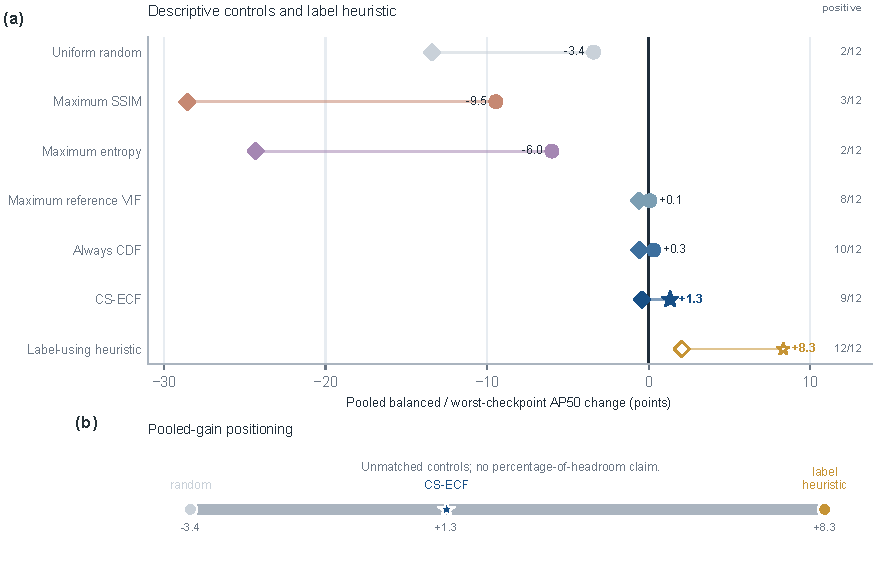
\includegraphics[width=\linewidth]{figures/FigureS1_controls_heuristic.pdf}
\caption{Exploratory image-statistic, random and label-using controls.
The figure is retained for complete reporting but is not used to establish a
confidence-specific mechanism. Source data are provided in
\texttt{FigureS1\_controls\_source.csv}.}
\label{fig:supp-controls}
\end{figure}

\begin{figure}[p]
\centering
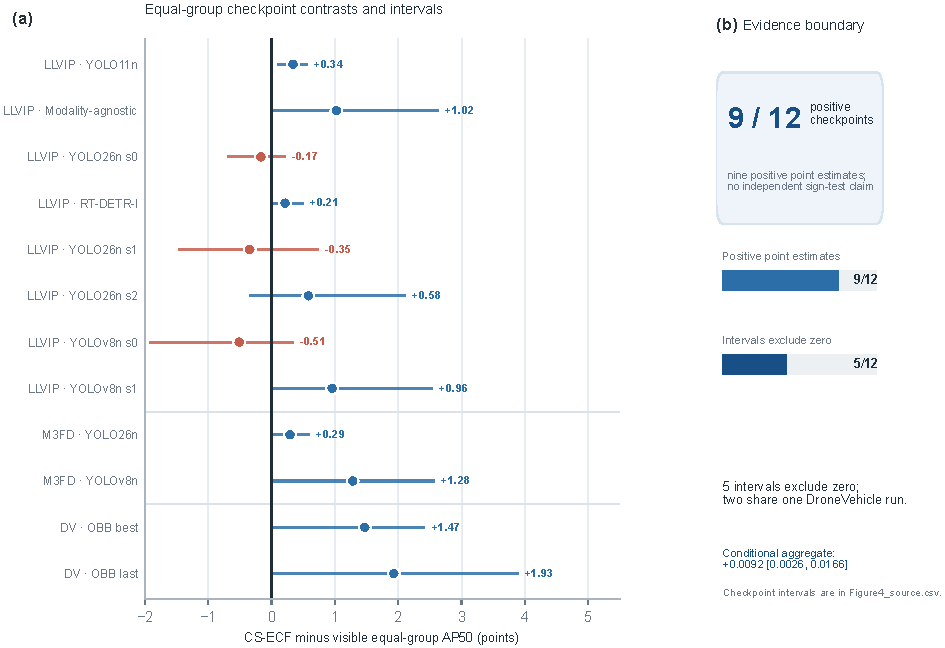
\includegraphics[width=\linewidth]{figures/FigureS2_checkpoint_intervals.pdf}
\caption{Checkpoint-level visible-relative contrasts and conditional
group-resampling intervals. These results provide the complete retrospective
screen but are not used as prospective confirmatory evidence. Source data are
provided in \texttt{FigureS2\_checkpoint\_source.csv}.}
\label{fig:supp-checkpoints}
\end{figure}

\begin{figure}[p]
\centering
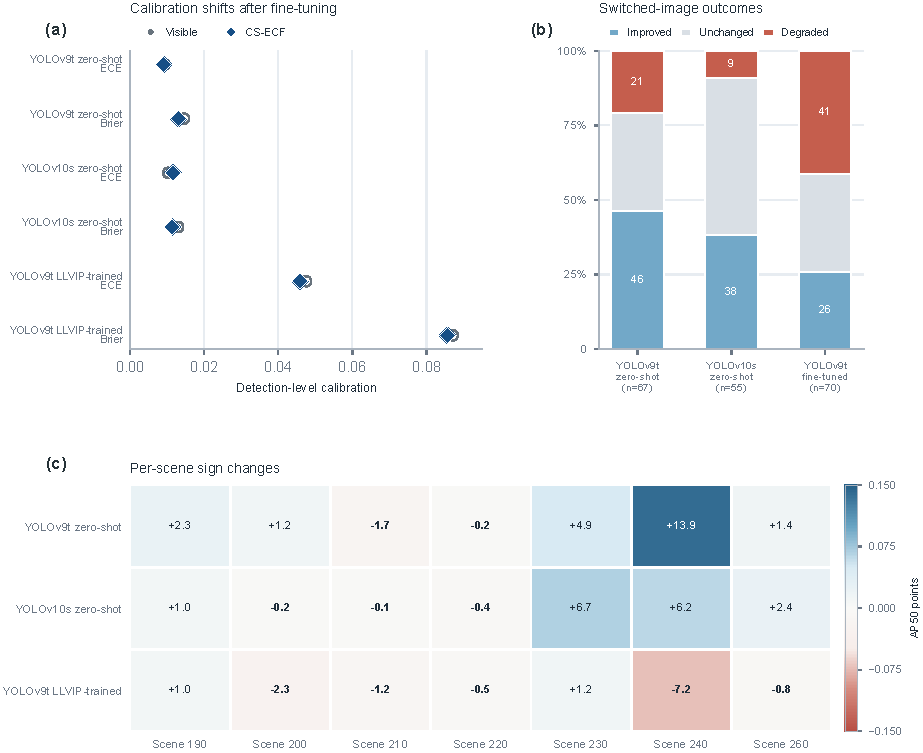
\includegraphics[width=\linewidth]{figures/FigureS3_calibration_boundary.pdf}
\caption{Calibration and switched-image diagnostics for the external
evaluators. The larger calibration error and higher degradation rate of the
fine-tuned checkpoint are consistent with a portability failure, but the
design does not establish causality. Source data are provided in
\texttt{FigureS3\_calibration\_source.csv}.}
\label{fig:supp-calibration}
\end{figure}

\begin{figure}[p]
\centering
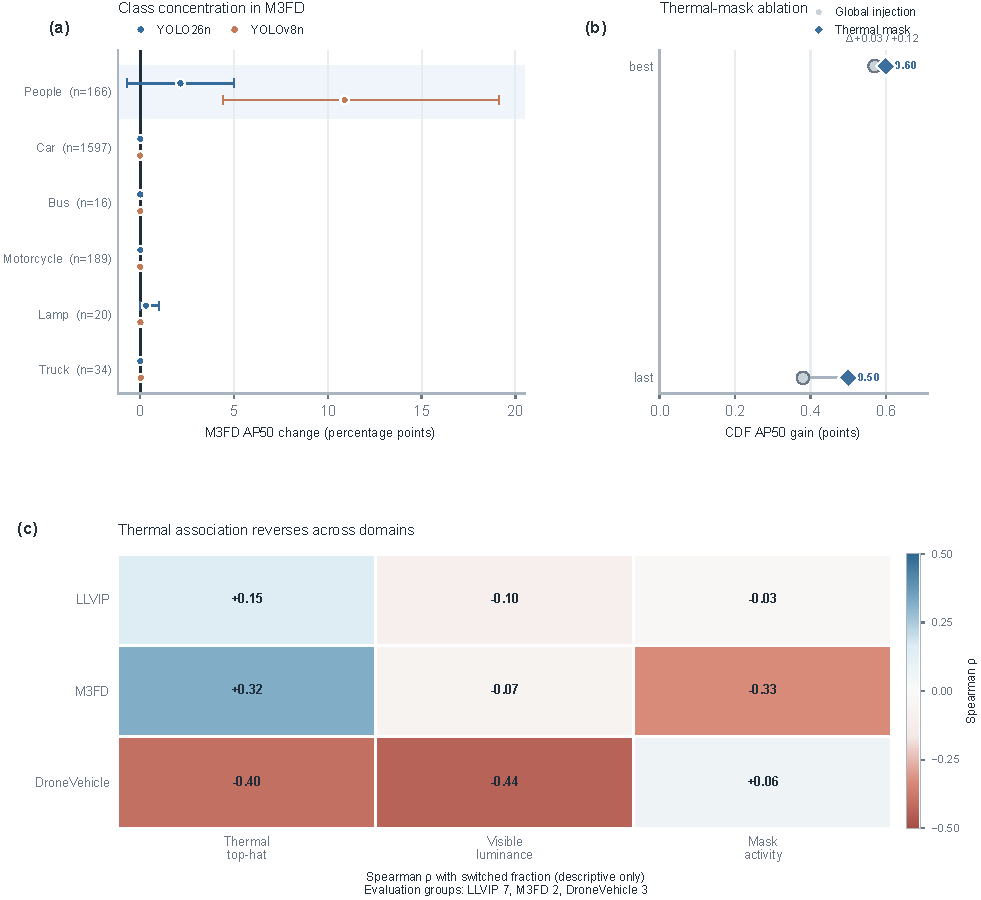
\includegraphics[width=\linewidth]{figures/FigureS4_thermal_class_boundary.pdf}
\caption{Class concentration and thermal-feature boundaries. The M3FD gain is
strongly concentrated in the people class, and the thermal association changes
sign across domains. Source data are provided in
\texttt{FigureS4\_thermal\_class\_source.csv}.}
\label{fig:supp-thermal}
\end{figure}

\begin{figure}[p]
\centering
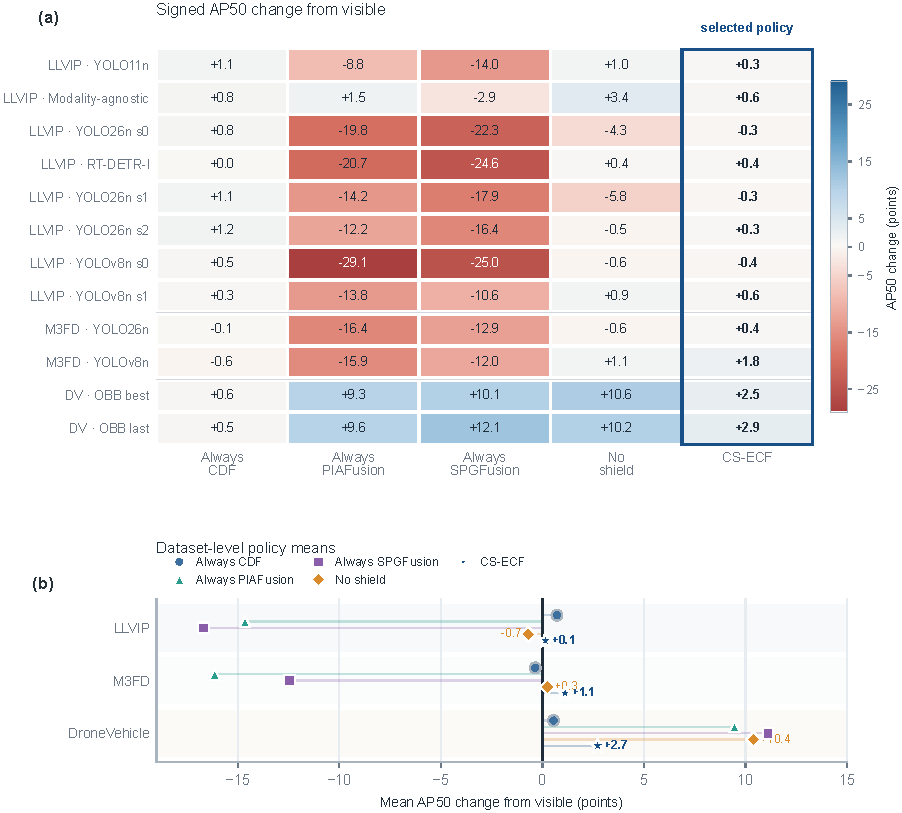
\includegraphics[width=0.92\linewidth]{figures/FigureS5_evaluator_dependence.pdf}
\caption{Retrospective evaluator-dependent utility across all fusion
candidates and checkpoints. The figure is retained as development evidence and
is not treated as the prospective effect estimate. Source data are provided in
\texttt{FigureS5\_evaluator\_source.csv}.}
\label{fig:supp-evaluator}
\end{figure}

\begin{figure}[p]
\centering
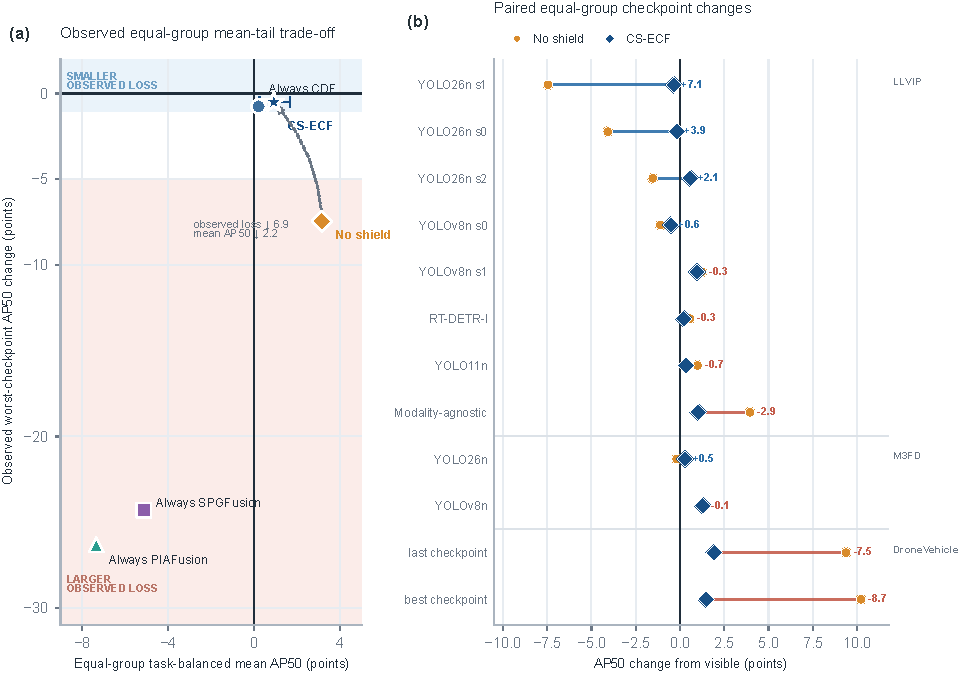
\includegraphics[width=0.90\linewidth]{figures/FigureS6_observed_tail_tradeoff.pdf}
\caption{Observed mean-tail trade-off under the no-shield selector and
CS-ECF. This is an empirical summary, not a future risk guarantee. Source data
are provided in \texttt{FigureS6\_tail\_source.csv}.}
\label{fig:supp-tail}
\end{figure}

\begin{figure}[p]
\centering
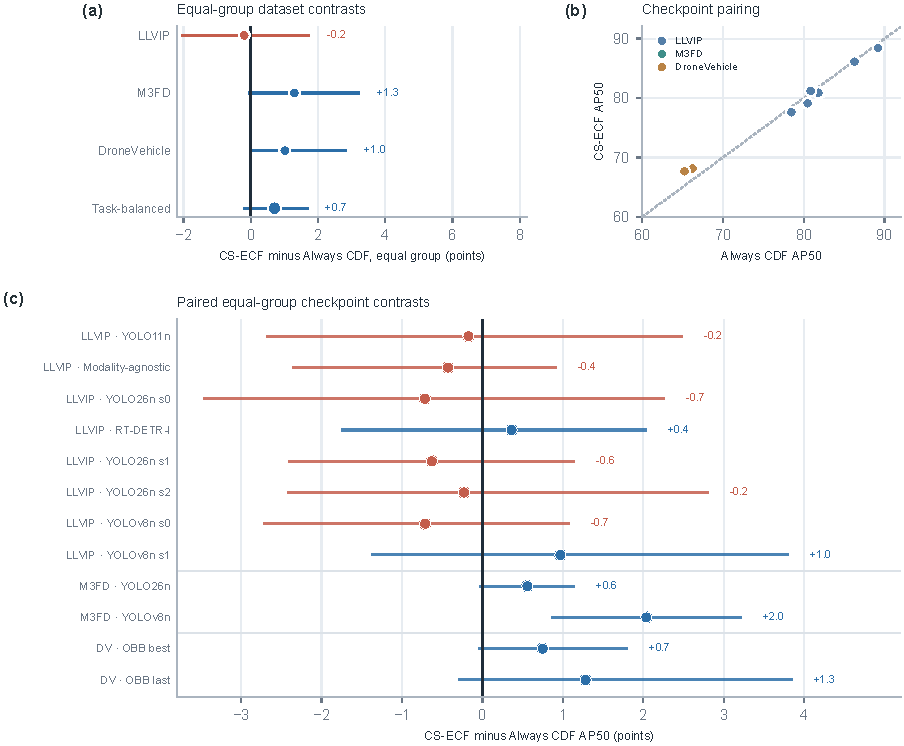
\includegraphics[width=0.90\linewidth]{figures/FigureS7_cdf_comparison.pdf}
\caption{Complete retrospective 12-checkpoint comparison of CS-ECF and Always
CDF. The held-out LLVIP and VEDAI contrasts are reported in
Table~\ref{tab:prospective-llvip} and Table~\ref{tab:vedai-supp} rather than
this retrospective panel. Source data are provided in
\texttt{FigureS7\_cdf\_source.csv}.}
\label{fig:supp-cdf}
\end{figure}

\begin{figure}[p]
\centering
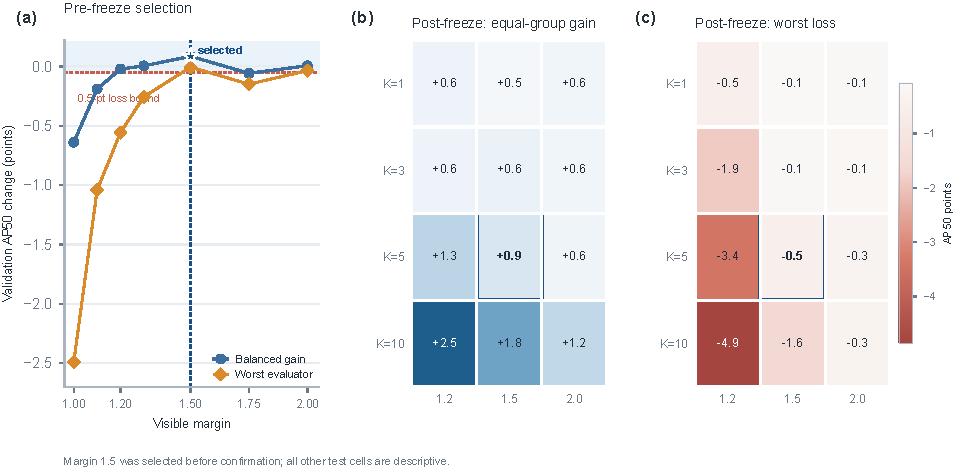
\includegraphics[width=0.94\linewidth]{figures/FigureS8_selection_sensitivity.pdf}
\caption{Development threshold selection and post-freeze sensitivity. Panel
(\textbf{a}) shows the original validation search over visible margins for
\(K=5\). Panels (\textbf{b},\textbf{c}) show equal-group test sensitivity over
score depth and margin. These diagnostics did not reselect the policy. Source
data are provided in \texttt{FigureS8\_selection\_source.csv}.}
\label{fig:supp-selection}
\end{figure}

\small
\section{Reproduction}

The repository contains the selector, candidate-generation and detector-scoring
code, per-image score arrays, full LLVIP, M3FD, DroneVehicle, and VEDAI
manifests, native OBB scoring, prospective protocol hashes, source data for
every figure, and scripts that reproduce the intervals. The prospective analysis environment was Python
3.10.22, NumPy 2.2.6, PyTorch 2.14.0 with CUDA 12.6, SciPy 1.15.3, and
Ultralytics 8.4.189.

The canonical equal-group analysis is generated by:

\begin{verbatim}
python analysis/cs_ecf/equal_group_statistics.py \
  --out results/major_revision/equal_group_statistics.json
\end{verbatim}

The pooled diagnostic script and the merge step are:

\begin{verbatim}
python scripts/analyze_csecf_vs_cdf.py
python analysis/cs_ecf/merge_equal_group_evidence.py \
  --equal results/major_revision/equal_group_statistics.json \
  --paired results/selective_fusion/csecf_vs_cdf_paired.json \
  --major results/major_revision/major_revision_statistics.json \
  --drone-combined results/evidence/dronevehicle_test_combined.json
\end{verbatim}

The pooled values remain under explicit \texttt{pooled\_} keys. Split and candidate
manifests retain their seeds and selected groups. The margin and score-depth
sensitivity analysis is reproduced by:

\begin{verbatim}
python analysis/cs_ecf/major_revision_statistics.py \
  --data-root "$SSGF_DATA_ROOT" --out results/revision_statistics.json
\end{verbatim}

The prospective LLVIP analyses and canonical evidence assembly are:

\begin{verbatim}
python reproduction/prospective_llvip_analysis.py \
  --root evidence/prospective \
  --data-root "$SSGF_DATA_ROOT" \
  --out evidence/prospective/llvip_primary_analysis.json
python reproduction/analyze_llvip_original_checkpoint_confirmation.py \
  --root evidence/prospective \
  --data-root "$SSGF_DATA_ROOT" \
  --out evidence/prospective/llvip_original8_analysis.json
python reproduction/assemble_prospective_evidence.py
python reproduction/canonicalize_external_evaluator_evidence.py
\end{verbatim}

The confidence-ordered matching sensitivity and its switch-budget-matched
control are regenerated by:

\begin{verbatim}
python reproduction/rescore_prospective_standard_matching.py
python reproduction/analyze_standard_matching_sensitivity.py
python reproduction/rescore_vedai_standard_matching.py
python reproduction/analyze_matched_switch_control.py \
  --evidence-root evidence/prospective_standard_matching \
  --out evidence/prospective_standard_matching/matched_switch_target_control.json
\end{verbatim}

The budgeted candidate-library analysis, transfer checks, and figure are
regenerated by:

\begin{verbatim}
python reproduction/budgeted_candidate_selection.py
python reproduction/plot_budgeted_candidate_selection.py
\end{verbatim}

The prospective visible-plus-PIA confirmation and measured end-to-end
pipeline are regenerated by:

\begin{verbatim}
python reproduction/fetch_pia_holdout.py
python reproduction/prepare_pia_sources.py
python reproduction/generate_pia_candidates.py
python reproduction/score_pia_confirmation.py
python reproduction/analyze_pia_confirmation.py
python reproduction/assemble_pia_confirmation.py
python reproduction/benchmark_end_to_end.py
python reproduction/summarize_end_to_end.py
\end{verbatim}

The CDF sensitivity candidates are generated one configuration at a time by
\texttt{reproduction/generate\_consensus\_detail.py}. After scoring each
candidate directory on the six-class M3FD evaluators, the packaged score arrays
and sensitivity table are summarized by:

\begin{verbatim}
python reproduction/analyze_cdf_sensitivity.py
\end{verbatim}

The complete M3FD split and external-evaluator score manifests are generated
by:

\begin{verbatim}
python reproduction/build_m3fd_split_manifest.py
python reproduction/package_external_evaluator_scores.py
\end{verbatim}

Image-statistics controls, external-evaluator diagnostics, and registration
quartiles use
\path{analysis/cs_ecf/image_quality_baselines.py},
\path{analysis/cs_ecf/external_evaluator_diagnostics.py}, and
\path{analysis/cs_ecf/alignment_csecf_sensitivity.py}, respectively. The image
quality script requires \texttt{--external-root} for the image directories.
M3FD class counts and contribution shares are generated by
\path{analysis/cs_ecf/summarize_m3fd_classes.py}.
Native DroneVehicle scoring and analysis use
\path{reproduction/score_dronevehicle_native_obb.py} and
\path{reproduction/analyze_dronevehicle_native_obb.py}. Independent training
uses \path{reproduction/prepare_dronevehicle_obb_runs.py} and
\path{reproduction/train_dronevehicle_obb_independent.py}. The archive includes
the exact protocol, per-image true-positive arrays, candidate-score summaries,
run manifests, and native score files needed to re-aggregate the reported OBB
intervals.

VEDAI preparation, training, native OBB scoring, analysis, and canonical
evidence assembly use \path{reproduction/prepare_vedai_obb.py},
\path{reproduction/train_vedai_obb.py},
\path{reproduction/score_vedai_native_obb.py},
\path{reproduction/analyze_vedai_native_obb.py}, and
\path{reproduction/assemble_vedai_evidence.py}, respectively. The package
includes the protocol hash, original-fold manifest, detector manifests,
per-image score arrays, and all positive and negative outcomes.

\end{document}
